% 1977 年河南卷第八题(3)：f1(x)=-1/4(x-1)^2+3（开口向下，实线）
% 与 f2(x)=1/4(x-1)^2+1（开口向上，虚线）的略图（按源卷第 4 页布局：x 轴 -1..4，y 轴刻度 1、2、3）
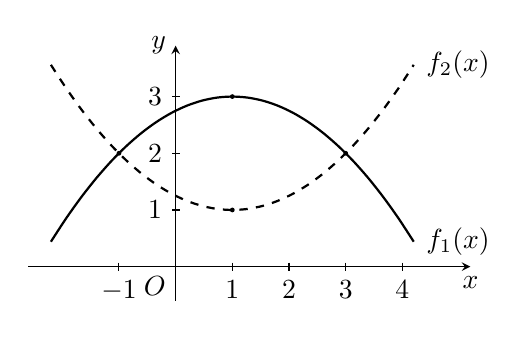
\begin{tikzpicture}[scale=0.72,>=stealth]
  \draw[->] (-2.6,0)--(5.2,0) node[below] {$x$};
  \draw[->] (0,-0.6)--(0,3.9) node[left] {$y$};
  \node[below left] at (0,0) {$O$};
  \foreach \x in {-1,1,2,3,4}{
    \draw[thin] (\x,0.07)--(\x,-0.07) node[below] {$\x$};
  }
  \foreach \y in {1,2,3}{
    \draw[thin] (0.07,\y)--(-0.07,\y) node[left] {$\y$};
  }
  \draw[thick,domain=-2.2:4.2,smooth] plot (\x,{-0.25*(\x-1)*(\x-1)+3});
  \draw[thick,dashed,domain=-2.2:4.2,smooth] plot (\x,{0.25*(\x-1)*(\x-1)+1});
  \fill (1,3) circle (1.2pt);
  \fill (1,1) circle (1.2pt);
  \fill (-1,2) circle (1.2pt);
  \fill (3,2) circle (1.2pt);
  \node[right] at (4.25,0.44) {$f_1(x)$};
  \node[right] at (4.25,3.56) {$f_2(x)$};
\end{tikzpicture}
